\documentclass[12pt, leqno]{article} %% use to set typesize
\input{common}

\usepackage{fontspec}
\usepackage{polyglossia}
\setmonofont{DejaVu Sans Mono}[Scale=MatchLowercase]
\usepackage[outputdir=pdf]{minted}

\providecommand{\tightlist}{%
  \setlength{\itemsep}{0pt}\setlength{\parskip}{0pt}}
\begin{document}



\hdr{2023-04-10}

\section{Nonlinear least squares}

Today we consider a special class of optimization problems: nonlinear
least squares. Given \(f : \mathbb{R}^n \rightarrow \mathbb{R}^m\) for
\(m > n\), we seek to minimize the objective function
\[\phi(x) = \frac{1}{2} \|f(x)\|^2.\] Differentiating gives us the
critical stationarity condition
\[\forall \delta x \in \mathbb{R}^n, \delta \phi(x) = f(x)^T f'(x) \delta x = 0;\]
or, equivalently, \[0 = \nabla \phi(x) = f'(x)^T f(x) = J(x)^T f(x).\]

Like linear least squares, nonlinear least squares problems often arise
from model fitting. Some important special cases include

\begin{itemize}
\tightlist
\item
  Separable problems of the form \(f(x, y) = \Phi(y) x - b\)
\item
  Linear models with nonlinear loss functions, where
  \(f_j(x) = \psi((Ax-b)_j)\)
\end{itemize}

For this lecture, let's consider three small example problems: one
general nonlinear least squares problem, one separable problem, and one
robust regression problem involving a nonlinear loss function. We will
use these examples to illustrate different ways we can use problem
structure -- and also show how to think about initial guesses.

\section{Newton and Gauss-Newton}

The Hessian of \(\phi\) is
\[H_{\phi}(x) = J(x)^T J(x) + \sum_{i=0}^m f_i(x) H_{f_i}(x)\] and while
it is certainly possible to run an ordinary Newton iteration for the
optimization problem, we can also note that the second term is
potentially small in the case when we can solve to a small residual
(i.e.~when \(f(x)\) gets close to zero). Hence, we consider the
\emph{Gauss-Newton} iteration, a scaled gradient descent iteration with
the scaling matrix \(J(x)^T J(x)\), i.e. \begin{align*}
  x^{k+1}
  &= x^k - \left[ J(x^k)^T J(x^k) \right]^{-1} J(x^k)^T f(x^k) \\
  &= x^k - J(x^k)^\dagger f(x^k)
\end{align*} As long as \(J\) remains nonsingular, the Gauss-Newton
direction is a descent direction. And assuming \(J\) is Lipschitz with
constant \(L\) near a stationary point \(x^*\), one can derive an error
iteration
\[\|e^{k+1}\| \leq L \|J(x^*)^\dagger\|^2 \|f(x^*)\| \|e^k\| + O(\|e^k\|^2)\]
This is an upper bound, but it suggests (accurately) that Gauss-Newton
is not guaranteed to converge even from small initial error. At the same
time, convergence can be very rapid for well-behaved problems
(\(J(x^*)\) not too near singular, Lipschitz constant is not too big)
when the residual norm at the solution is small. If \(f(x^*) = 0\), we
recover the same type of quadratic convergence we see for Newton's
method.

\begin{minted}{julia}
function gauss_newton(fJ, x0; rtol=1e-8, maxiter=100,
                      monitor=(x, rnorm)->nothing)
    x = copy(x0)
    for k = 1:maxiter
	fx, Jx = fJ(x)
	rnorm = norm(Jx'*fx)
	monitor(x, rnorm)
	if norm(Jx'*fx) < rtol
	    return x
	end
	x -= Jx\fx  # Solves the least squares update
    end
    error("Did not reach convergence in $maxiter iterations")
end
\end{minted}

\begin{minted}{julia}
gauss_newton(f, J, x0; rtol=1e-8, maxiter=100, monitor=(x, rnorm)->nothing) =
    gauss_newton((x)->(f(x), J(x)), x0,
                 rtol=rtol, maxiter=maxiter, monitor=monitor)
\end{minted}

\subsubsection{Questions}

\begin{enumerate}
\def\labelenumi{\arabic{enumi}.}
\tightlist
\item
  Show how to write one Gauss-Newton step in terms of a linear least
  squares problem.
\item
  Suppose \(m = n\). What does Gauss-Newton look like in this case?
\item
  Justify the claim that if \(J\) is nonsingular, the Gauss-Newton
  direction is a descent direction.
\end{enumerate}

\subsection{A reaction rate example}

This example is taken from
\href{https://en.wikipedia.org/wiki/Gauss\%E2\%80\%93Newton_algorithm\#Example}{Wikipedia}
and involves fitting the chemical reaction rate for an enzyme mediated
reaction. The larger the substrate concentration of the enzyme
(\([S]\)), the faster the rate of reaction \(R\), according to a
relation of the form \[R = \frac{V_{\max} [S]}{K_M + [S]}\] Writing the
unknowns as \(\beta = \begin{bmatrix} V_{\max} & K_M \end{bmatrix}^T\),
we solve the nonlinear least squares problem \[\mbox{minimize } 
  \sum_i \left( R_i - \frac{\beta_1 S_i}{\beta_2 + S_i} \right)^2\] over
a collected data set. To get an initial guess, we multiply each residual
by \(\beta_2 + S_i\) to solve the ordinary least squares problem
\[\mbox{minimize } \sum_i \left( (\beta_2 + S_i) R_i - \beta_1 S_i \right)^2\]

\begin{minted}{julia}
# Biological reaction-rate model fitting problem from Wikipedia
biox_f, biox_J, biox_H, biox_β0 = let

    # Data set
    S = [0.038; 0.194; 0.425; 0.626;  1.253;  2.500;  3.740]
    R = [0.050; 0.127; 0.094; 0.2122; 0.2729; 0.2665; 0.3317]
    
    # Residual function and Jacobian
    f(β) = R-β[1]*S ./ (β[2] .+ S)
    J(β) = [-S./(β[2] .+ S)  β[1]*S./(β[2] .+ S).^2]
    
    # Hessian function
    function H(β)
	Hβ = J(β)'*J(β)
	fβ = f(β)
	for j = 1:length(fβ)
	    Hβ += fβ[j] *
                [0.0                   S[j]/(β[2]+S[j])^2           ;
		 S[j]/(β[2]+S[j])^2   -2.0*β[1]*S[j]/(β[2] + S[j])^3]
	end
	Hβ
    end
    
    # Initial guess based on R(β[2] + S) ≈ β[1]*S
    β0 = [S -R]\(R .* S)
    
    f, J, H, β0
    
end
\end{minted}

According to the Wikipedia article, the true parameters are about
\(\hat{\beta}_1 = 0.362\) and \(\hat{\beta}_2 = 0.556\); a quick sanity
check reassures us that we have a good initial guess from the linear
least squares problem.

\begin{figure}
\begin{center}
  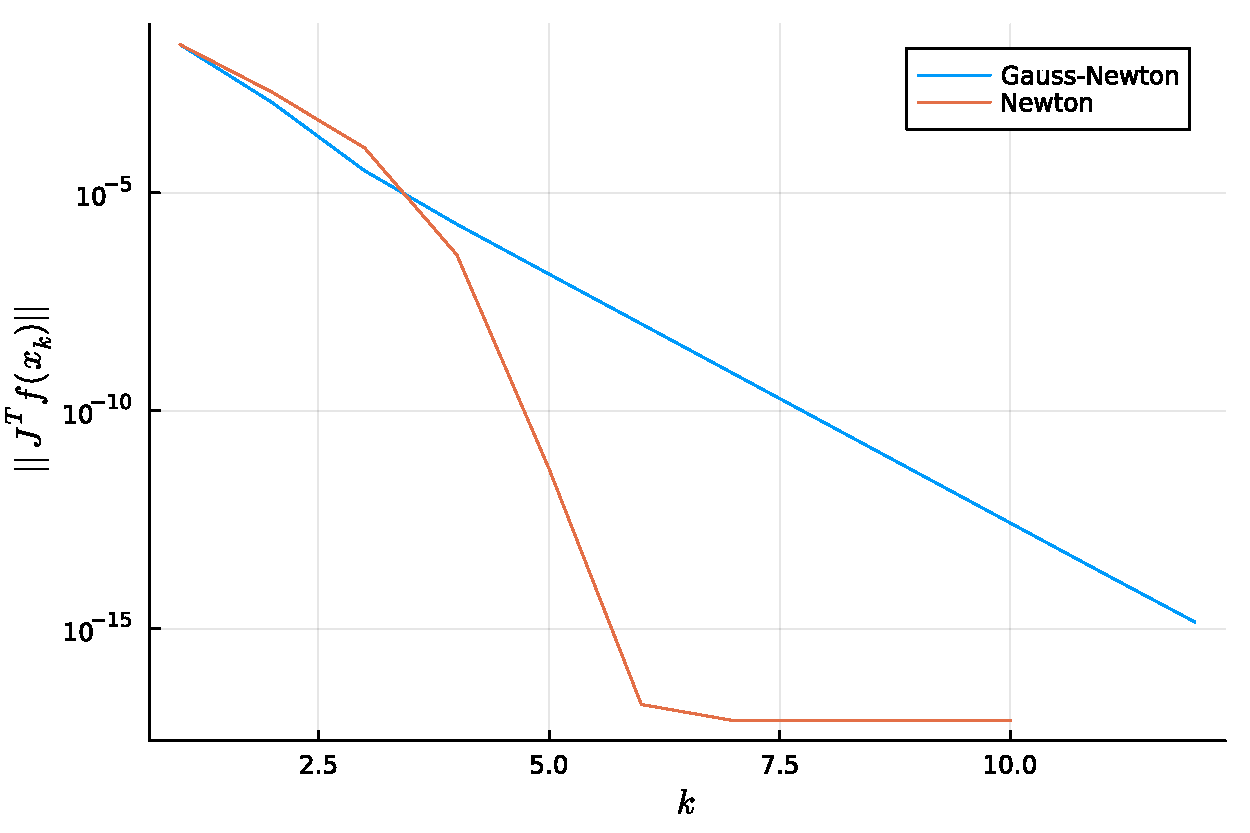
\includegraphics[width=0.8\textwidth]{fig/2023-04-10-biox-cvg.pdf}
\end{center}
\caption{Convergence of Gauss-Newton and Newton for a biological reaction
  rate fitting example.}
\label{fig:biox-cvg}
\end{figure}

Let's apply both Gauss-Newton and Newton to solve the problem.
We show the convergence of the two iterations in Figure~\ref{fig:biox-cvg}.

\begin{minted}{julia}
let
    biox_resids = []
    biox_β_gn =
        gauss_newton(biox_f, biox_J, biox_β0, rtol=1e-14, 
		     monitor=(x, rnorm)->push!(biox_resids, rnorm))
    p = plot(biox_resids, yscale=:log10,
	 ylabel="\$||J^T f(x_k)||\$", xlabel="\$k\$", label="Gauss-Newton")

    biox_resids_n = []
    biox_β = copy(biox_β0)
    for j = 1:10
	push!(biox_resids_n, norm(biox_J(biox_β)'*biox_f(biox_β)))
	biox_β -= biox_H(biox_β)\(biox_J(biox_β)'*biox_f(biox_β))
    end
    plot!(biox_resids_n[biox_resids_n .> 0], label="Newton")
md"""
- Gauss-Newton computed ($(biox_β_gn[1]), $(biox_β_gn[2]))
- Newton computed ($(biox_β[1]), $(biox_β[2]))

$p
"""
end
\end{minted}

Compared to the Newton iteration, Gauss-Newton is getting (fast) linear
convergence, and ends up taking about twice as many iterations to drive
the residual down close to \(10^{-15}\). At the same time, Gauss-Newton
doesn't require that we form the Hessian matrix!

\subsection{An actual bound for Gauss-Newton (optional)}

We are not going to do the actual error iteration for Gauss-Newton
iteration in class, but it is not that conceptually difficult -- it's
just that the algebra is a bit tedious. We'll keep it in the notes for
the sake of completeness.

In the interest of keeping the notation concise, let's write
\(J^* = J(x^*)\) and \(J_k = J(x^k) = J_* + E_k\). Similarly, let
\(f_* = f(x^*)\). We assume throughout the derivation that \(J\) is
Lipschitz with constant \(L\) (in the 2-norm) and that
\(\sigma_{\min}(J_*) > L \|e^k\|\), implying that
\[\sigma_{\min}(J_k) \geq 
  \sigma_{\min}(J_*) - \|E_k\| \geq \sigma_{\min}(J_*)-L\|e^k\| > 0.\]
By the fundamental theorem of calculus,
\[f(x^k) = f_* + \int_0^1 J(x+\xi e^k) e^k d\xi\] Therefore we can write
\(p^k = -J_k^\dagger f(x^k)\) as \[p^k = -(J_k^T J_k)^{-1} J_k^T f_* 
  -J_k^\dagger \int_0^1 J(x+\xi e^k) e^k \, d\xi\] Using the fact that
\(J_*^T f_* = 0\) (by stationarity), we have
\[-(J_k^T J_k)^{-1} J_k^T f_* = -(J_k^T J_k)^{-1} E_k^T f_*,\] which
gives us the bound \[\|-(J_k^T J_k)^{-1} J_k^T f_*\| \leq 
  \frac{L \|f^*\| \|e^k\|}{\left( \sigma_{\min}(J_*)-L\|e^k\| \right)^2}.\]
and using the fact that \(J_k^\dagger J_k = I\) (assuming \(J_k\) full
rank), we have \[-J_k^\dagger \int_0^1 J(x+\xi e^k) e^k \, d\xi = 
  -e^k -J_k^\dagger \int_0^1 (J(x+\xi e^k)-J_k) e^k \, d\xi,\] and by
the Lipschitz condition and consistency,
\[\|-J_k^\dagger \int_0^1 (J(x+\xi e^k)-J_k) e^k \, d\xi\|
  \leq \frac{L\|e^k\|^2}{2(\sigma_{\min}(J_*)-L\|e^k\|)}\] Substituting
these bounds into \(e^{k+1} = e^k + p^k\), we have \[\|e^{k+1}\| \leq 
    L \left( \frac{\|f^*\|}{(\sigma_{\min}(J_*)-L\|e^k\|)^2} +
             \frac{\|e^k\|/2}{\sigma_{\min}(J_*)-L\|e^k\|} \right) \|e^k\|\]
and if \(L \|f_*\|/\sigma_{\min}(J_*)^2 < 1\) then a sufficient
condition for error to decrease by some \(\alpha < 1\) (where \(\alpha\)
does not depend on \(e^k\)) is
\[\|e^k\| \leq \frac{2\sigma_{\min}(J_*)}{5L} 
  \left( 1 - \frac{L\|f_*\|}{\|\sigma_{\min}(J_*)\|^2} \right)\] and so
the Gauss-Newton iteration is guaranteed to converge if
\[\|e^k\| \leq \frac{2\sigma_{\min}(J_*)}{5L} 
  \left( 1 - \frac{L\|f_*\|}{\|\sigma_{\min}(J_*)\|^2} \right)\]

\section{Levenberg-Marquardt}

Gauss-Newton can converge quite quickly under some circumstances, but
suffers when

\begin{itemize}
\tightlist
\item
  The minimal residual is large
\item
  The Jacobian is close to singular
\item
  The Lipschitz constant on \(J\) is large
\end{itemize}

There is not much we can do about \(\|f(x_*)\|\) or about the Lipschitz
constant on the Jacobian. But we do know how to deal with
ill-conditioned least squares problems! The Levenberg-Marquardt
algorithm replaces the least squares solve in the Gauss-Newton algorithm
with a regularized least squares solve:
\[x^{k+1} = x^k - (J_k^T J_k + \lambda^2 D_k^2)^{-1} J_k^T f(x^k)\] The
scaling matrix \(D_k\) may be an identity (suggested by Levenberg) or a
diagonal matrix whose diagonal entries are the column norms of \(J_k\)
(suggested by Marquardt).

When \(\lambda\) approaches zero, the Levenberg-Marquardt step
approaches the Gauss-Newton step. As \(\lambda\) becomes large, it
approaches a small scaled gradient step with the scaling matrices
\(D_k\). Unlike Gauss-Newton, we can always get Levenberg-Marquardt to
converge given a good enough initial guess and a large enough
\(\lambda\). In practice, though, we usually choose \(\lambda\)
adaptively. We'll return to how we do this in another lecture.

\begin{minted}{julia}
function levenberg_marquardt(fJ, x0; λ = 1e-3, rtol=1e-8, maxiter=100,
                             monitor=(x, rnorm)->nothing)
    x = copy(x0)
    for k = 1:maxiter
	fx, Jx = fJ(x)
	d = sqrt.(sum(Jx.^2, dims=1))
	rnorm = norm(Jx'*fx)
	monitor(x, rnorm)
	if norm(Jx'*fx) < rtol
	    return x
	end
	x -= [Jx; sqrt(λ)*diagm(d[:])]\[fx; zeros(length(x))]
    end
    error("Did not reach convergence in $maxiter iterations")
end
\end{minted}

\begin{minted}{julia}
levenberg_marquardt(f, J, x0; λ = 1e-3, rtol=1e-8, maxiter=100, 
		    monitor=(x, rnorm)->nothing) =
    levenberg_marquardt((x)->(f(x), J(x)), x0, λ=λ, rtol=rtol,
                        maxiter=maxiter, monitor=monitor)
\end{minted}

\subsubsection{Questions}

\begin{enumerate}
\def\labelenumi{\arabic{enumi}.}
\tightlist
\item
  Justify the claims about the asymptotic behavior of
  Levenberg-Marquardt as \(\lambda\) approaches 0 and \(\infty\).
\item
  Explain the implementation of the Levenberg-Marquardt step in the
  code.
\end{enumerate}

\subsection{A peak-fitting example}

In various types of spectroscopy, one sees ``peaks'' in frequency space
associated with different types of resonances. A
\href{https://en.wikipedia.org/wiki/Cauchy_distribution}{Lorentzian}
peak (also known as a Breit-Wigner peak or a Cauchy distribution) with
center \(x_0\), width parameter \(\Gamma\), and amplitude parameter
\(c\) has the form
\[\frac{c}{\pi} \frac{\Gamma/2}{(x-x_0)^2 + (\Gamma/2)^2}.\] Our problem
here is to fit empirical measurements to a sum of Lorentzian peaks. This
problem occurs often enough that there are specific approaches people
take (we wouldn't always treat this as a general nonlinear least squares
problem), but we will only take advantage of the partially linear nature
of the problem, i.e.~that we are minimizing
\[\sum_j \left( y_j - \sum_i \phi(x_j; x_{c,i}, \Gamma_i) c_i \right)^2\]
where \(\phi(x_j; x_{c,i}, \Gamma_i)\) is the value at \(x_j\) of the
Lorentzian peak with amplitude one at center \(x_{c,i}\) and with scale
parameter \(\Gamma_i\). That is, the amplitudes are determined by a
\emph{linear} least squares problem in which the coefficient matrix
depends on some other parameters.

\begin{minted}{julia}
# Lorentzian peak-finding problem
lorx_fJ, lorx_ΦJ, lorx_yy, lorx_p0, lorx_plot = let

    # Reference peak locations, widths, and amplitudes
    xc_ref = [0.5; 1.3; 1.5]
    Γs_ref = [0.3; 0.1; 0.1]
    cs_ref = [0.6; 1.0; 0.8]
    
    # Reference signal function -- combination of Lorentzians
    ϕref(x, xc, Γs) = Γs/(2π) ./ ((x.-xc).^2 .+ (0.5*Γs).^2)
    
    # Generate noisy signal
    xx = range(0.0, 2.0, length=100)
    yy = [ϕref(x, xc_ref, Γs_ref)'*cs_ref for x in xx] 
    yy += 5e-2 * randn(100)
    
    # Residual and Jacobian
    function fJresid(xc, Γ, c)
	resid = copy(yy)
	J = zeros(100,9)
	for k = 1:3
            
	    f     = -c[k]*Γ[k]/(2π)
	    df_dΓ = -c[k]/(2π)
	    df_dc = -Γ[k]/(2π)
            
	    g      = (xx.-xc[k]).^2 .+ (0.5*Γ[k])^2
	    dg_dxc = -2*(xx.-xc[k])
	    dg_dΓ  = 0.5*Γ[k]
            
	    resid += f./g
	    J[:,k]   = -f./g.^2 .* dg_dxc
	    J[:,k+3] = (df_dΓ.*g .- f.*dg_dΓ)./g.^2
	    J[:,k+6] = df_dc./g
            
	end
	resid, J
    end
    
    # Basis vectors and derivatives with respect to xc and Γ
    function ΦJmatrix(xc, Γ)
	Φ = zeros(100,3)
	J = zeros(100,6)
	for k = 1:3
            
	    f     = Γ[k]/(2π)
	    df_dΓ = 1.0/(2π)
            
	    g      = (xx.-xc[k]).^2 .+ (0.5*Γ[k])^2
	    dg_dxc = -2*(xx.-xc[k])
	    dg_dΓ  = 0.5*Γ[k]
            
	    Φ[:,k]   = f./g
	    J[:,k]   = -f./g.^2 .* dg_dxc
	    J[:,k+3] = (df_dΓ.*g .- f.*dg_dΓ)./g.^2
            
	end
	Φ, J
    end
    
    # Residual and Jacobian as functions of p = [xc, Γ, c]
    fJp(p) = fJresid(p[1:3], p[4:6], p[7:9])
    
    # Basis and Jacobian as functions of [xc, Γ]
    ΦJp(p) = ΦJmatrix(p[1:3], p[4:6])
    
    # Initial guess
    p0 = [0.5; 1.2; 1.6; 0.2; 0.2; 0.2; 1.0; 1.0; 1.0]
    
    # Plotting function
    function lorx_plot(p)
	plot(xx, yy, label="Signal")
	plot!(xx, yy-fJp(p)[1], style=:dash, label="Approximation")
    end
    
    fJp, ΦJp, yy, p0, lorx_plot
end
\end{minted}

\begin{figure}
\begin{center}
  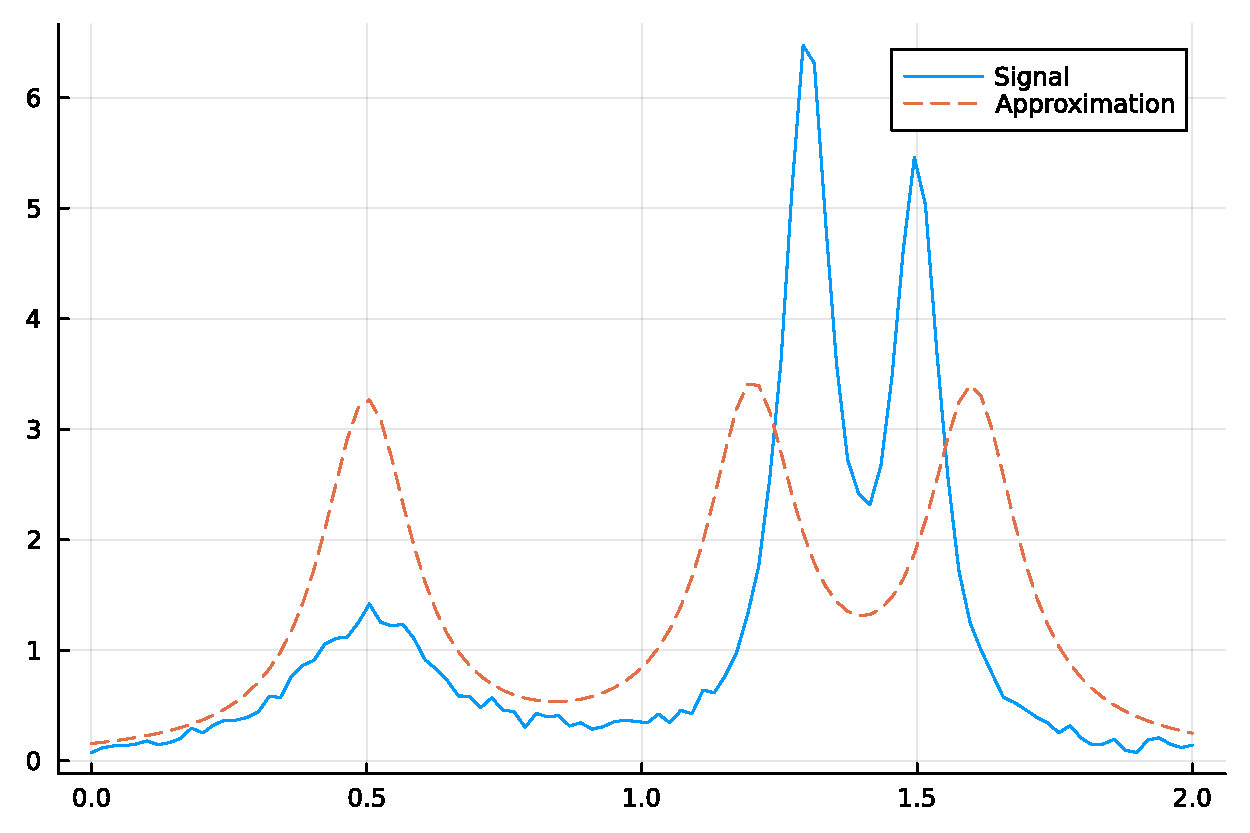
\includegraphics[width=0.8\textwidth]{fig/2023-04-10-lorx_guess.pdf}
\end{center}
\caption{Initial guess for Lorentzian fitting example.}
\label{fig:lorx-guess}
\end{figure}

\begin{figure}
\begin{center}
  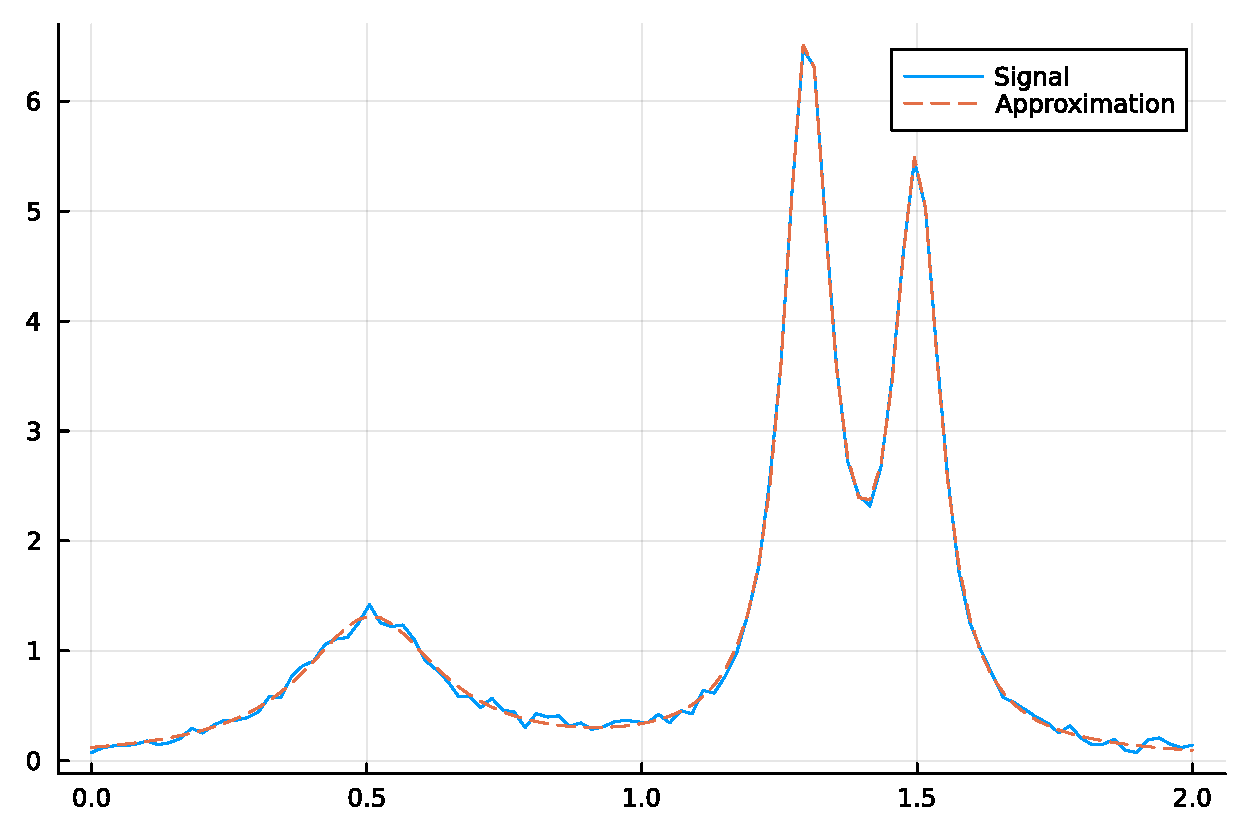
\includegraphics[width=0.8\textwidth]{fig/2023-04-10-lorx_lm.pdf}
\end{center}
\caption{Converged solution for Lorentzian fitting example.}
\label{fig:lorx-lm}
\end{figure}

\begin{figure}
\begin{center}
  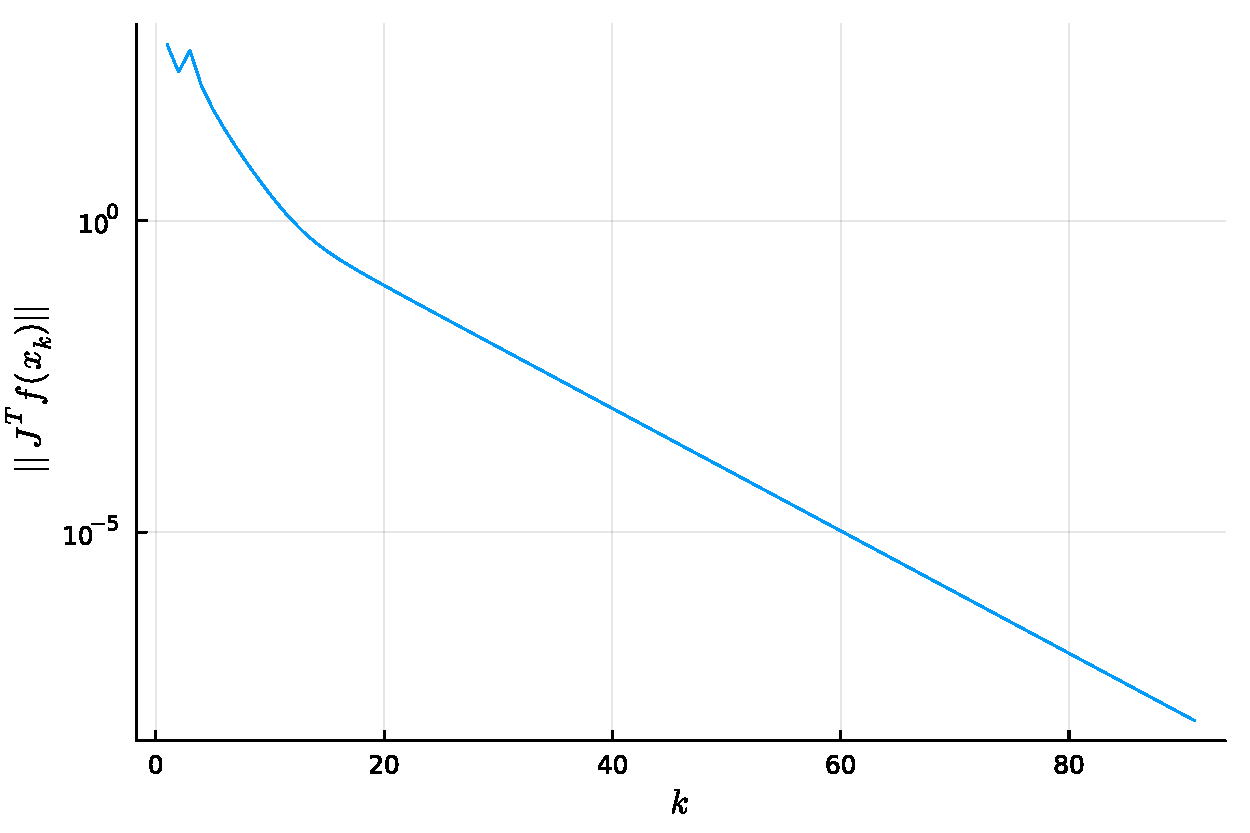
\includegraphics[width=0.8\textwidth]{fig/2023-04-10-lorx_lm_cvg.pdf}
\end{center}
\caption{Convergence of Levenberg-Marquardt for Lorentzian fitting example.}
\label{fig:lorx-lm-cvg}
\end{figure}

We start with a not-fantastic initial guess
(Figure~\ref{fig:lorx-guess}).  Getting a good initial guess is
actually an interesting problem, but one that we will not address
here.  The converged solution is shown in Figure~\ref{fig:lorx-lm},
and the convergence history in Figure~\ref{fig:lorx-lm-cvg}.  From
this initial guess, Gauss-Newton does not have any hope of
convergence, but Levenberg-Marquardt does.

\subsubsection{Questions}

\begin{enumerate}
\def\labelenumi{\arabic{enumi}.}
\tightlist
\item
  Play with the parameter \(\lambda\) in the Levenberg-Marquardt call.
  What happens?
\item
  Play with the initial guess. Does convergence improve from a better
  starting guess?
\item
  Argue that the ``true'' signal looks like \(p(x)/q(x)\) for low degree
  polynomials \(p\) and \(q\), where \(q\) has complex roots
  \(x_{c,i} \pm \iota \Gamma_i/2\). We can find \(p\) and \(q\) by
  setting \(p(x_i) - y_i q(x_i) \approx 0\) in a least squares sense;
  how would we implement this directly to get a better initial guess for
  the centers and widths of the Lorentzians?
\end{enumerate}

\section{Variable projection}

In the Lorentzian peak-fitting example, our function \(f\) had the form
\[f(x_c, \Gamma, c) = y-\Phi(x_c, \Gamma) c.\] But if we know the
centers and width parameters, then computing the amplitude parameters
becomes a standard linear least squares problem. Putting in the solution
gives us the reduced problem (or \emph{projected} problem)
\[f_{\mathrm{proj}}(x_c, \Gamma) = 
  \left( I-\Phi(x_c, \Gamma) \Phi(x_c, \Gamma)^\dagger \right) y = Py\]
where \(P = I-\Phi \Phi^\dagger\) is the residual projector. The reduced
problem can then be solved with any of our nonlinear least-squares
solvers. This technique, known as variable projection, is
\href{http://stacks.iop.org/IP/19/R1}{widely used in a variety of
applications}.

Minimizing the norm of \(f_{\mathrm{proj}}\) is often nicer than
minimizing the norm of the original \(f\). Of course, in order to do
this, we need to be able to compute the Jacobian of
\(f_{\mathrm{proj}}\)! Fortunately, we have lots of experience at this
point with computing such derivatives. Using the definition of the
pseudoinverse and mumbling over algebra for a while yields:
\begin{align*}
  \delta P &= 
  -(\delta \Phi) \Phi^\dagger - (\Phi^\dagger)^T (\delta \Phi)^T
  + (\Phi^\dagger)^T (\Phi^T \delta \Phi + (\delta \Phi)^T \Phi) \Phi^\dagger \\
  &= -P (\delta \Phi) \Phi^\dagger - (\Phi^\dagger)^T (\delta \Phi)^T P \\
  \delta f_{\mathrm{proj}} &= (\delta P) y 
  = -P (\delta \Phi) c - (\Phi^\dagger)^T (\delta \Phi)^T r
\end{align*} where \(c = \Phi^\dagger y\) and
\(r = f_{\mathrm{proj}} = y - \Phi c\). Given the full QR decomposition
\[\Phi = 
  \begin{bmatrix} Q_1 & Q_2 \end{bmatrix} 
  \begin{bmatrix} R_1 \\ 0 \end{bmatrix}\] and observing that
\(P = I-Q_1 Q_1^T = Q_2 Q_2^T\) and \((\Phi^\dagger)^T = Q_1 R_1^{-T}\),
we have \[\delta f_{\mathrm{proj}} 
  = -Q_2 Q_2^T (\delta \Phi) c - Q_1 R^{-T} (\delta \Phi)^T r \\
  = -Q 
  \begin{bmatrix} 
    R^{-T} (\delta \Phi)^T r \\ 
    Q_2^T (\delta \Phi) c 
  \end{bmatrix}\]

We know that the Householder QR factorization stores \(Q\) implicitly,
and while we can apply \(Q\) and \(Q^T\) quickly, we probably do not
want to explicitly form \(Q_2\). But we can evaluate the above
expression without explicitly forming \(Q_2\) by

\begin{itemize}
\tightlist
\item
  Forming \(Q^T (\delta \Phi) c\)
\item
  Overwriting the leading rows with \(R^{-T} (\delta \Phi)^T r\)
\item
  Multiplying the result by \(Q\)
\item
  Negating the whole thing
\end{itemize}

In the case of the peak-finding problem, each of the parameters affects
only one basis vector. So, for example
\[\frac{\partial f_{\mathrm{proj}}}{\partial x_{c,j}}
  = -Q 
  \begin{bmatrix} R^{-T} e_j
    \left( \frac{\partial \phi_j}{\partial x_{c,j}} \right)^T r \\ 
    Q_2^T \left(\frac{\partial \phi_i}{\partial x_{c,j}}\right) c_j 
  \end{bmatrix}\] and similarly for the derivatives with respect to the
width parameters \(\Gamma_j\).

\begin{minted}{julia}
function lorx_fJproj(p)
    Φ, JΦ = lorx_ΦJ(p)
    F = qr(Φ)
    
    # Compute c and r (aka f_proj)
    QTyy = F.Q'*lorx_yy
    c = F.R\QTyy[1:3]
    QTyy[1:3] .= 0.0
    r = F.Q*QTyy
    
    # Compute W = -Q'*Jf_proj via the above
    W = (F.Q'*JΦ) .* [c; c]'
    z = JΦ'*r
    invRT = inv(F.R')
    W[1:3,1:3] = invRT .* z[1:3]'
    W[1:3,4:6] = invRT .* z[4:6]'
    
    # Return f_proj and the Jacobian of f_proj
    r, -(F.Q * W)
end
\end{minted}

\begin{figure}
\begin{center}
  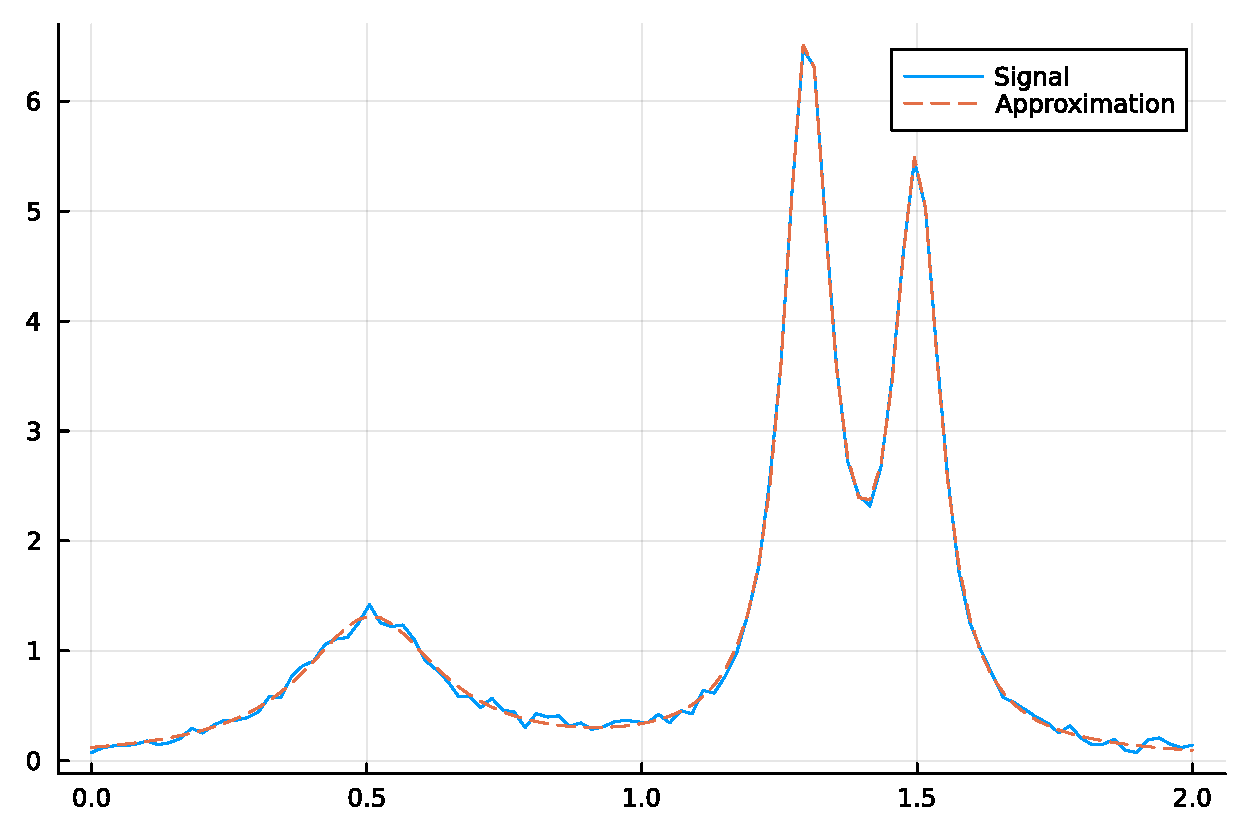
\includegraphics[width=0.8\textwidth]{fig/2023-04-10-lorx_vproj.pdf}
\end{center}
\caption{Converged solution for Lorentzian fitting example with 
  variable projection formulation.}
\label{fig:lorx-vproj}
\end{figure}

\begin{figure}
\begin{center}
  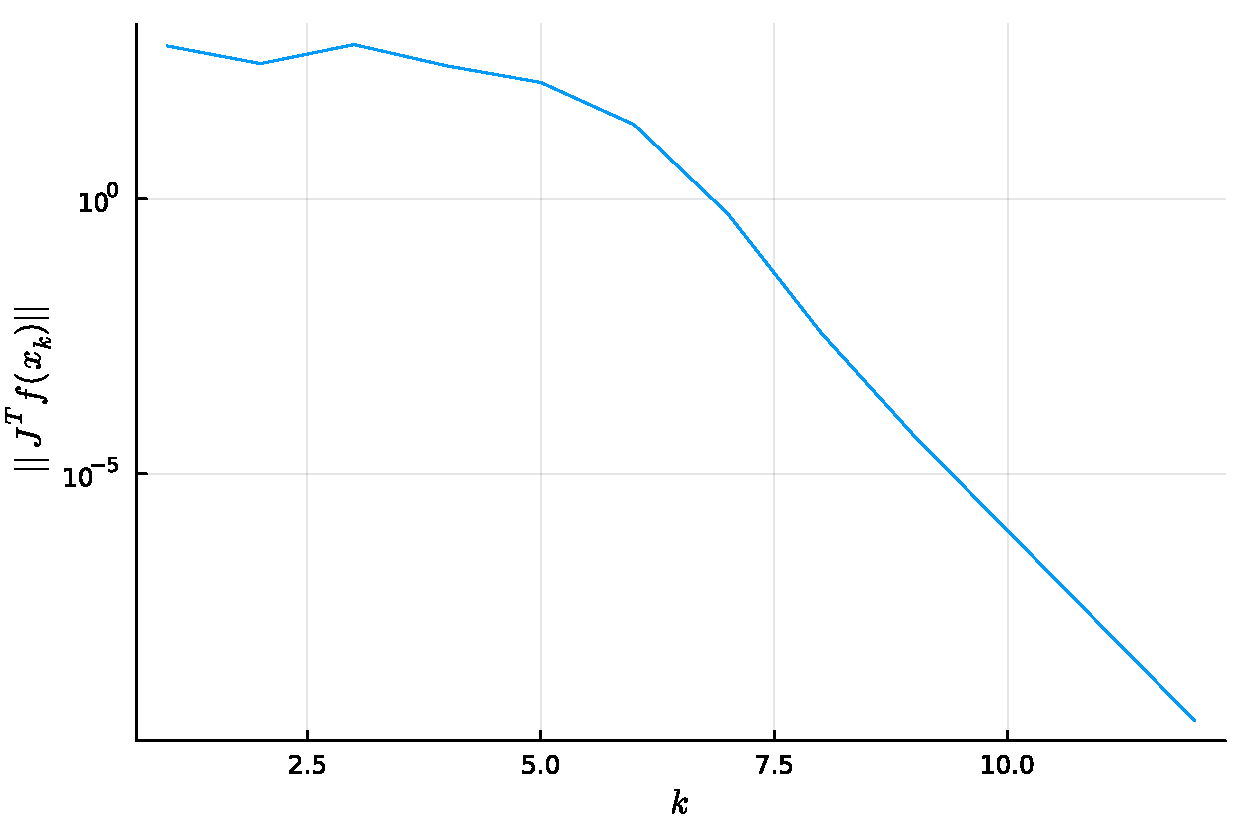
\includegraphics[width=0.8\textwidth]{fig/2023-04-10-lorx_vproj_cvg.pdf}
\end{center}
\caption{Convergence of Gauss-Newton for variable projection formulation of
  Lorentzian fitting example.}
\label{fig:lorx-vproj-cvg}
\end{figure}

Unlike the original full problem, the projected version of the problem can be
solved rather quickly with Gauss-Newton, even if we use our not-so-fantastic
initial guess.  The converged solution is shown in Figure~\ref{fig:lorx-vproj};
we show the convergence plot in Figure~\ref{fig:lorx-vproj-cvg}.

\subsubsection{Questions}

\begin{enumerate}
\def\labelenumi{\arabic{enumi}.}
\tightlist
\item
  Can you derive the expression for \(\delta P\) yourself?
\item
  Explain the expression for the derivative of \(f_{\mathrm{proj}}\)
  with respect to \(x_{c,i}\).
\item
  We claimed that \(P = I-Q_1 Q_1^T = Q_2 Q_2^T\); why are these two
  expressions equivalent?
\end{enumerate}

\section{Iteratively reweighted least squares}

A number of optimization problems from statistics have the form
\[\mbox{minimize } \phi(x) = \sum_{i=1}^m \rho(r_i), \quad r = Ax-b.\]
where we will assume \(\rho\) is an even function with \(\rho(0) = 0\).
This can, of course, be converted to a nonlinear least squares problem,
but we will stick with this form. Let \(\psi\) denote the derivative of
\(\rho\); then we have \begin{align*}
  \nabla \phi(x) &= A^T \psi(r) \\
  H_{\phi}(x) &= A^T \operatorname{diag}(\psi'(r)) A
\end{align*} where \(\psi(r)\) and \(\psi'(r)\) should be interpreted
elementwise. A Newton step for this problem is
\[p = -(A^T \operatorname{diag}(\psi'(r)) A)^{-1} A^T \psi(r)\] and this
is equivalent to solving the weighted least squares problem
\[\mbox{minimize } 
  \left\| 
    \frac{\psi(r)}{\psi'(r)} + Ap 
  \right\|_{\operatorname{diag}(\psi'(r))}^2\]

where \(\psi(r)/\psi'(r)\) should be interpreted elementwise.

Of course, we already know that Newton iteration is not globally
convergent in general, but this iteration has another irritating issue:
it is undefined when any component of \(\psi'(r)\) is exactly zero!
There are interesting cases where this is a real issue. However, an a
slight modification avoids this problem and \emph{is} globally
convergent for convex loss functions. Define \(W(f)\) to be the diagonal
matrix of weights \(w_k = \psi(r_k)/r_k\); then \(x\) is a stationary
point for \(\phi\) if \[A^T \psi(r) = A^T W(r) r = 0.\] This suggests
the fixed point iteration \[A^T W(r^k) r^{k+1} = 0,\] that is,
\[x^{k+1} = \operatorname{argmin} \|Ax-y\|_{W(r^k)}^2.\] In words, at
each step we compute a new weighted least squares fit to the data.
Observe that
\[w_k = \frac{\psi(r_k)}{r_k} = \frac{\psi(r_k)-\psi(0)}{r_k-0} =
  \psi'(r_k) + o(f_k)\] and
\[\frac{\psi(r_k)}{\psi'(r_k)} = \frac{\psi'(0) r_k}{\psi'(0)} +
  o(r_k) = r_k + o(r_k);\] hence, as with Gauss-Newton, this iteration
is similar to Newton iteration when the residuals are small.

This algorithm is an example of an \emph{iteratively reweighted least
squares} (IRLS) algorithm. Several algorithms share the IRLS name; all
have the property that each iterate is the solution to a weighted least
squares problem, where the weights vary from iteration to iteration.

\begin{minted}{julia}
function irls(A, b, x0, ψ; maxiter=100, rtol=1e-8,
              monitor=(x,rnorm)->nothing)
    x = copy(x0)
    for k = 1:maxiter
	r = A*x-b
	ψr = ψ.(r)
	rnorm = norm(A'*ψr)
	monitor(x, rnorm)
	if rnorm < rtol
	    return x
	end
	ws = sqrt.(ψr./r)
	ws[r .== 0] .= 0.0
	x = (ws .* A)\(ws .* b)
    end
end
\end{minted}

\subsubsection{Questions}

\begin{enumerate}
\def\labelenumi{\arabic{enumi}.}
\tightlist
\item
  Write the IRLS iteration in additive update form -- that is, what
  least squares problem does \(p^k = x^{k+1}-x^k\) satisfy? Compare to
  the Newton least squares problem.
\item
  Explain the line \texttt{ws{[}r\ .==\ 0{]}\ .=\ 0.0} in the
  \texttt{irls} routine.
\end{enumerate}

\subsection{Robust regression}

Least squares regression works well for Gaussian noise, but tends to
perform poorly in the presence of \emph{outliers}. Fitting procedures
that better tolerate outliers are generally known as \emph{robust
regression} procedures. The most popular robust regression techniques
involve solving a nonlinear least squares problem
\[\mbox{minimize } \sum_{j=1}^m \rho(r_j), \quad r = Ax-b\] for some
loss function \(\rho\) that grows more slowly than the squared loss. The
coefficients from this estimation procedure are known as
\href{https://en.wikipedia.org/wiki/M-estimator}{\(M\)-estimators}.

In order to compute \(M\)-estimators, we first want some initial guess
at the solution and at the typical level of (non-outlier) noise in the
data. A typical trick to do this is to draw random subsets of the data
until we think that with high probability we have at least one subset
that contains no outliers. For each subset, we do an ordinary least
squares fit, and then judge quality based on the
\href{https://en.wikipedia.org/wiki/Median_absolute_deviation}{median
absolute deviation (MAD)}, i.e.~the median absolute value of the
residuals. We return as our initial guess for \(x\) the solution that
has the smallest MAD. Based on the assumption that non-outlier data is
subject to normal noise, we also return a scale factor of MAD/0.6745
(since for the standard normal the expected value of the MAD is 0.6745).

\begin{minted}{julia}
# Estimate Ax ≈ b with outlier fraction ρ
function rr_init(A, b, ρ; nbatch=0, pfail=1e-6)
    m, n = size(A)
    nbatch = max(n, nbatch)
    
    # Scale factor based on median absolute deviation (MAD)
    s_mad(r) = median(abs.(r))/0.645
    
    # Number of trials such that
    #   P(all draws of size n include an outlier) < pfail
    # Analysis assumes m is sufficiently bigger than n that drawing
    # with or without replacement is about the same.
    ntrials = ceil(log(pfail)/log1p(-(1.0-ρ)^nbatch))
    
    # Fit to subsets of the data and take the solution with the
    # smallest median absolute deviation (MAD)
    xbest = zeros(n)
    mad_best = Inf
    for t = 1:ntrials
	s = randperm(m)[1:nbatch]
	x = A[s,:]\b[s]
	mad = median(abs.(b-A*x))
	if mad < mad_best
	    xbest[:] = x
	    mad_best = mad
	end
    end
    
    # Return best fit wrt MAD and estimated scale factor
    xbest, mad_best/0.6745
end
\end{minted}

Two of the most common loss functions used in robust regression are

\begin{itemize}
\tightlist
\item
  Huber loss: quadratic near the origin and then grows linearly away
  from the origin
\item
  Tukey loss: roughly quadratic near the origin, then flattens out to a
  constant
\end{itemize}

The Huber loss function is convex, and so the nonlinear least squares
problem with Huber loss has a unique solution. The Tukey loss is less
sensitive to extreme outliers, but may in general lead to many local
minimizers.

\begin{minted}{julia}
begin
    # Huber loss function and its derivatives
    huber(r, c) = if abs(r) < c 0.5*r^2 else c*(abs(r)-c/2) end
    dhuber(r, c) = if abs(r) < c r else c*sign(r) end
    
    # Tukey loss function and its derivatives
    tukey(r, c) = if abs(r) < c c^2/6*(1.0-(1.0-(r/c)^2)^3) else c^2/6 end
    dtukey(r, c) = if abs(r) < c r*(1.0-(r/c)^2)^2 else 0.0 end
end
\end{minted}

Now we set up and solve a robust regression problem with 10\% outliers,
using \texttt{rr\_init} to get an initial guess and the iteratively
weighted least squares procedure to optimize the Tukey loss with an
appropriately chosen scale factor.

\begin{minted}{julia}
# Robust regression / M-estimator example with Tukey biweight loss
rrx_results = let

    # Set up a least-squares type of problem with random data
    A = rand(200,3)
    xref = rand(3)
    b = A*xref + 5e-2 * randn(200)
    
    # Introduce some outliers
    b[50:60] .= 100.0
    
    # Get initialization
    x0, s = rr_init(A, b, 0.1)
    
    # Tukey loss with appropriate scale factor
    ρ(r) = tukey(r, 4.685*s)
    ψ(r) = dtukey(r, 4.685*s)
    
    # Run the IRLS algorithm
    resids = []
    x = irls(A, b, x0, ψ, rtol=1e-12, monitor=(x,rnorm)->push!(resids, rnorm))
    
    # Return scale factor, errors in initial guess and output, and residuals
    s, norm(x0-xref), norm(x-xref), resids
end
\end{minted}

\begin{figure}
\begin{center}
  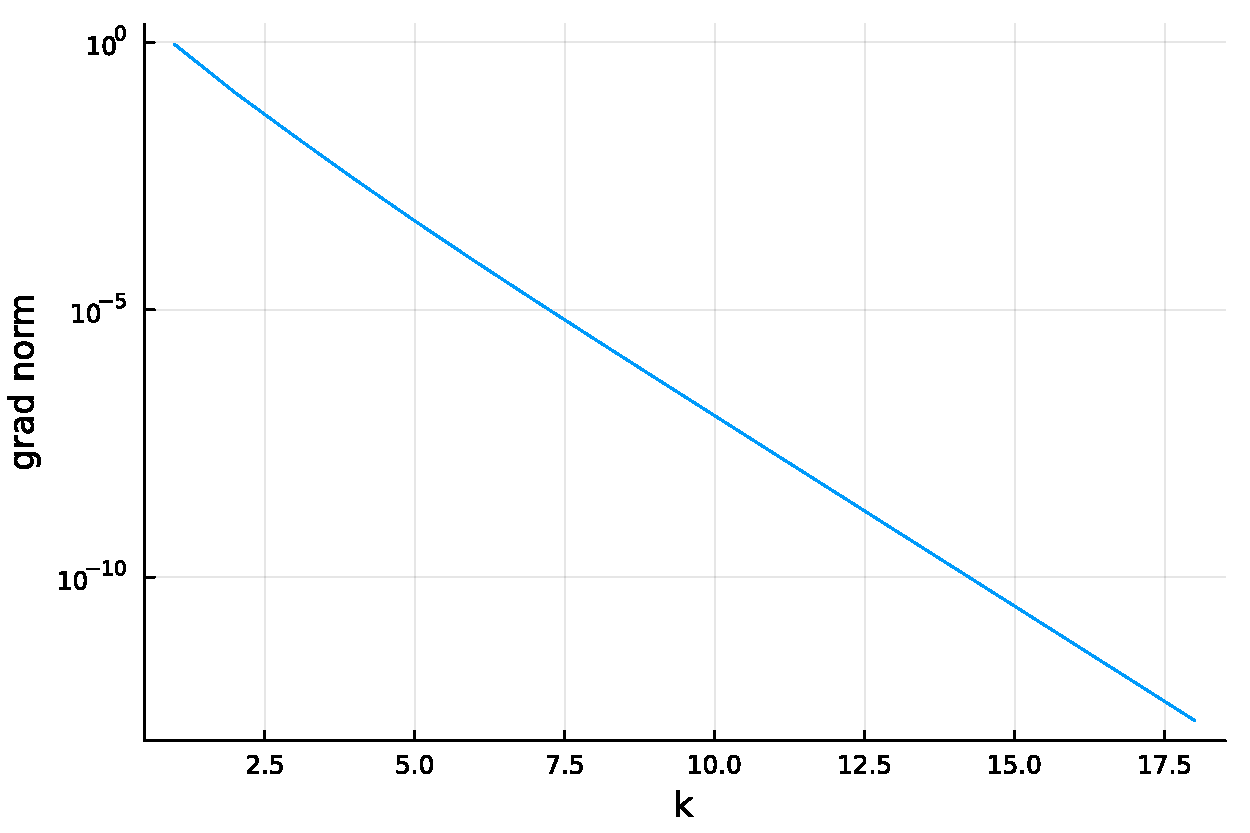
\includegraphics[width=0.8\textwidth]{fig/2023-04-10-rrx-cvg.pdf}
\end{center}
\caption{Convergence of IRLS.}
\label{fig:rrx-cvg}
\end{figure}

Running this example gives an initial estimate with error of
$0.033$ and an associated scale factor of
$0.052$.  
After 18 steps of IRLS,
we get a converged result with an estimation error of
$0.030$.

The convergence plot is shown in Figure~\ref{fig:rrx-cvg}.

\subsubsection{Questions}

\begin{enumerate}
\def\labelenumi{\arabic{enumi}.}
\tightlist
\item
  Will the \texttt{rr\_init} routine fail if we unluckily draw a subset
  such that \texttt{As{[}s,:{]}} is singular?
\item
  Plot \(\psi(r)/r\) at the converged solution. Explain what you
  observe.
\end{enumerate}


\end{document}
